\chapter{Theoretical Background}\label{chapter:basis}


\section{Trajectory Planning Problem}

\begin{figure}[htpb]
      \centering
      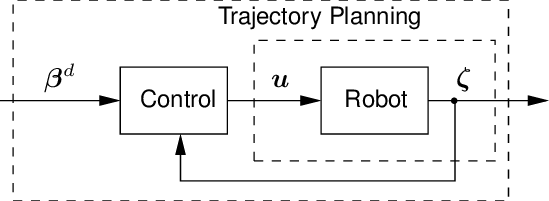
\includegraphics[width=0.5\textwidth]{figures/trajectory_planning.png}
      \caption{Trajectory planning in the closed loop control system}
      \label{fig:trajectory-loop}
\end{figure}

In order to execute a task of cleaning whiteboard we need to come with the algorithms that will generate us the movement of robotic arm. Generally speaking if we have two points we can create a line or an arc that will connect those points. 

Having this in mind, the first family of algorithms that will be $point-to-point$ transitional functions. These functions will typically receive as an timestamp, or relative clock $t$ from the start till the end of trajectory generation. Moreover, typically the program is specified by the constraints such as desired velocity $q'_max$ and applied acceleration $q''$ which define the shape of the path and the type of movement that is planned (fast, slow, linear, etc.). Depending on the application those algorithms might be really complex, for such task as whiteboard cleaning we need the simplest linear/rotational movements. 

\section{Trajectory Profile - Trapezoidal velocity}

\begin{figure}[htpb]
    \centering
    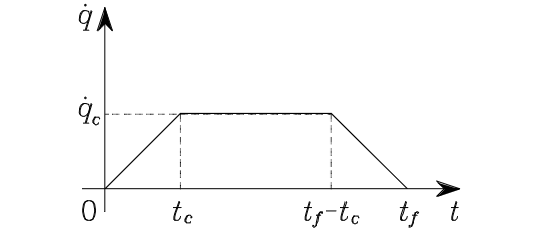
\includegraphics[width=0.5\linewidth]{trap-profile.png}
    \caption{Trapezoidal velocity profile}
    \label{fig:trapezoidal-profile}
\end{figure}

The first task was to make the so called velocity profile. According to the Robotics: Modelling, Planning and Control \parencite{robotics_book} the easiest solution which enforces constant absolute value of $q''$  is \textbf{trapezoidal velocity profile}. The practicality of this solution comes from the real life hardware constraints, where the robot cannot immediately reach the maximum speed and needs to accelerate to it. Same goes for the deceleration. In the figure \autoref{fig:trapezoidal-profile} it is shown explicitly. 

The formulae for finding the position using constant* acceleration can be described according to the \parencite{robotics_book} is: 
\[
q(t) = \begin{cases}
    q_i + \frac{1}{2} \ddot{q}_c t^2 &  0 \le t \le t_c \\
    q_i + \ddot{q}_c t_c \left( t - \frac{t_c}{2} \right) &  t_c \le t \le t_f - t_c \\
    q_f - \frac{1}{2} \ddot{q}_c (t_f - t)^2 & t_f - t_c \le t \le t_f
\end{cases}
\] 
where: 

\begin{enumerate}
    \item $t$ is the current time, and $t_c$  is time needed to reach maximum $\dot{q}$. Finally $t_f$ is the overall time needed for executing the program.
    \item $q_i$ is the current position which we are updating, $q_f$ is the final position
    \item  $\ddot{q}_c$ is the absolute value of the constant acceleration
\end{enumerate}

Moreover, we simplify the model, by just considering one degree of freedom. This way we can later, add up multiple velocity profile for the same joint, if other coordinates would need to be changed, instead of just trying to handle multiple cases of different coordinates at the same place in the code. 

\section{Trajectory Generation in 3D}

After having a mathematical model for the 1D velocity profile, we can think of how to generate a path of movement. Since, typically, user is defining its desired start and end position, these would be our parameters into the function to generate the point in 3D space. More formally we can say: 
$$
p = f([ \sigma_{start}, \sigma_{end} ])
$$

where $\sigma_{start}$ and $\sigma_{end}$ are the start and end desired positions. 
\break

There are two primitive ideas to generate a path from one point to the other, which are 
\begin{itemize}
\item Linear movement  
\item Circular movement  
\end{itemize}

From these primitive movements we can potentially create more complex patterns of robot locomotion.

\subsection{Rectilinear movement} 
Even though the textbook of rectilinear movement describes more sophisticated patterns that this type can create, our case is a simple linear path generation from a to b. This is why the formula applied is the same, the parameters can be strictly defined and are described below

\[
\textbf{p} = \textbf{p}_i + s * \frac{ \textbf{p}_f - \textbf{p}_i }{ 
\left\| \textbf{p}_f - \textbf{p}_i \right\| }
\]

Let us explore this formula. It essentially tells us which direction we will move by specifying the difference between current($\textbf{p}_i$) and end points ($\textbf{p}_f$). We divide this vector of direction with the norm and multiply by the rate of change $s$ that we have of our trajectory. Since, the trajectory for the linear movement doesn't change such $s$ can be a predefined as the difference between start and end position, resulting in:

\[
\textbf{p} = \textbf{p}_0 + 2 * \frac{ \textbf{p}_f - \textbf{p}_0 }{ 
\left\| \textbf{p}_f - \textbf{p}_i \right\| }
\]

where $\textbf{p}_0$ is the starting point of the trajectory. This way simplified the generalized solution for our purpose.

\subsection{Circular path}

When simulating circular motion, it is possible to interpolate the previous rectilinear trajectory. However, a much nicer solution is use the notion of unit circle and angles between the start and endpoint. Even though in the original textbook \parencite{robotics_book} there is a  more expressive solution, we have decided to stick to the simpler formula. 

\[
\mathbf{p}(s) = 
\begin{pmatrix}
    \rho \cos \left(\frac{s}{\rho}\right) \\
    \rho \sin \left(\frac{s}{\rho}\right) \\
    0
\end{pmatrix}
\]

Essentially what we are doing is assigning to the $x$ and $y$ coordinates their position relative to the unit circle. To grasp all circles, the notion of radius is added $\rho$. Also $x$ is defined though the cosine of the angle, same for the $y$, just we are using sine instead. 






% The goal of trajectory genera is to create an input (can have multiple parameters but in a broad sense its usually current position $q$, velocity $q'$ and acceleration $q''$). T
% Trajectory planning according to ~\parencite{robotics_book}.

% \section{Section}
% Citation test (with Biber)~\parencite{latex}.

% \subsection{Subsection}

% See~\autoref{tab:sample}, \autoref{fig:sample-drawing}, \autoref{fig:sample-plot}, \autoref{fig:sample-listing}, \autoref{fig:tum}, \autoref{fig:tumslide}.

% \begin{table}[htpb]
%   \caption[Example table]{An example for a simple table.}\label{tab:sample}
%   \centering
%   \begin{tabular}{l l l l}
%     \toprule
%       A & B & C & D \\
%     \midrule
%       1 & 2 & 1 & 2 \\
%       2 & 3 & 2 & 3 \\
%     \bottomrule
%   \end{tabular}
% \end{table}

% \begin{figure}[htpb]
%   \centering
%   % This should probably go into a file in figures/
%   \begin{tikzpicture}[node distance=3cm]
%     \node (R0) {$R_1$};
%     \node (R1) [right of=R0] {$R_2$};
%     \node (R2) [below of=R1] {$R_4$};
%     \node (R3) [below of=R0] {$R_3$};
%     \node (R4) [right of=R1] {$R_5$};

%     \path[every node]
%       (R0) edge (R1)
%       (R0) edge (R3)
%       (R3) edge (R2)
%       (R2) edge (R1)
%       (R1) edge (R4);
%   \end{tikzpicture}
%   \caption[Example drawing]{An example for a simple drawing.}\label{fig:sample-drawing}
% \end{figure}

% \begin{figure}[htpb]
%   \centering

%   \pgfplotstableset{col sep=&, row sep=\\}
%   % This should probably go into a file in data/
%   \pgfplotstableread{
%     a & b    \\
%     1 & 1000 \\
%     2 & 1500 \\
%     3 & 1600 \\
%   }\exampleA
%   \pgfplotstableread{
%     a & b    \\
%     1 & 1200 \\
%     2 & 800 \\
%     3 & 1400 \\
%   }\exampleB
%   % This should probably go into a file in figures/
%   \begin{tikzpicture}
%     \begin{axis}[
%         ymin=0,
%         legend style={legend pos=south east},
%         grid,
%         thick,
%         ylabel=Y,
%         xlabel=X
%       ]
%       \addplot table[x=a, y=b]{\exampleA};
%       \addlegendentry{Example A};
%       \addplot table[x=a, y=b]{\exampleB};
%       \addlegendentry{Example B};
%     \end{axis}
%   \end{tikzpicture}
%   \caption[Example plot]{An example for a simple plot.}\label{fig:sample-plot}
% \end{figure}

% \begin{figure}[htpb]
%   \centering
%   \begin{tabular}{c}
%   \begin{lstlisting}[language=SQL]
%     SELECT * FROM tbl WHERE tbl.str = "str"
%   \end{lstlisting}
%   \end{tabular}
%   \caption[Example listing]{An example for a source code listing.}\label{fig:sample-listing}
% \end{figure}

% \begin{figure}[htpb]
%   \centering
%   
\includegraphics[width=0.8\textwidth]{figures/tum}
%   \caption{For pictures with the same name, the direct folder needs to be chosen.} \label{fig:tumslide}
% \end{figure}

% \begin{figure}[!tbp]
%   \centering
%   \subfloat[TUM Logo][The logo.]{
\includegraphics[height=0.2\textheight]{tum}\label{fig:tum1}}
%   \hfill
%   \subfloat[TUM Slide][The famous slide.]{
\includegraphics[height=0.2\textheight]{figures/tum}\label{fig:tum2}}
%   \caption{Two TUM pictures side by side.}
%   \label{fig:sidebyside}
% \end{figure}

% This is how the glossary will be used.

% \Glspl{ddye}, \gls{r0}, \gls{R0}, and \gls{kdeac}. Also, the \glspl{tum} has many \glspl{computer}, not only one \Gls{computer}. Subsequent acronym usage will only print the short version of \glspl{tuma} (take care of plural, if needed!), like here with \gls{tuma}, too. It can also be --> \glsdisp{tum}{hidden}\footnote{Example for a hidden TUM glossary entry.} <--.

% \todo{Now it is your turn to write your thesis.

% This will be a few tough weeks.}

% \done{Nevertheless, celebrate it when it is done!}
